\section{Labels buy speed, images buy accuracy}
\label{sec:trap}

\begin{figure}[t]
\centering
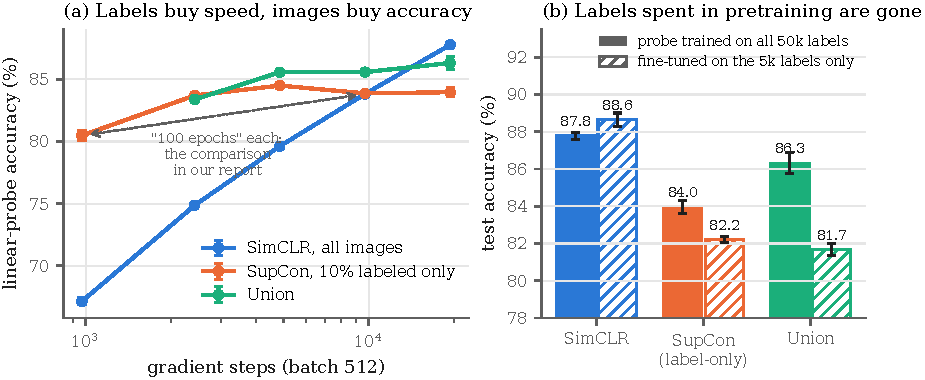
\includegraphics[width=\linewidth]{figures/fig_main.pdf}
\caption{\textbf{The two main results} (CIFAR-10, 10\% labels, ResNet-18, mean $\pm$ s.d.\ over seeds where
shown). \textbf{(a)} Linear-probe accuracy against the number of gradient steps, with every method given the
same steps. Label-only \supcon learns much faster but stops improving after about 5,000 steps; \simclr on all
images keeps improving and overtakes it. Our original report compared \supcon after 970 steps with \simclr
after 9,700 (``100 epochs'' each, dashed arrow) and concluded that the labels hurt.
\textbf{(b)} After 19,400 steps. Solid: probe trained on all 50,000 labels, the standard protocol. Hatched:
fine-tuned with the 5,000 labels that actually exist. Fine-tuning helps \simclr but not the encoders that
already used the same labels during pretraining.}
\label{fig:main}
\end{figure}

\subsection{The epoch trap}

Our report compared \supcon and \simclr at ``100--200 epochs'' each. With $N$ images and batch $B$, an epoch
is $\lfloor N/B\rfloor$ steps, so an epoch over the 5,000 labeled images is 9 steps and an epoch over the
50,000 images is 97. In the report, \supcon therefore received 900 gradient steps and \simclr 19,400, a
21-fold difference that we did not notice at the time.

\Cref{fig:main}a replays this comparison in our controlled setting. After 970 steps (``100 epochs'' over the
labeled images), label-only \supcon reaches \supconTenLinPm, \gapBudget points below \simclr after 9,700
steps (\simclrLinPm). The original report used a ResNet-50, which needs even more steps: trained for 970 steps
in our pipeline, a ResNet-50 \supcon reaches \rFiftySupconTen, within one point of the 75.2\% we reported
(\cref{tab:budget} in \cref{app:extra}). The original gap was therefore mostly a gap in training, not in
supervision.

\subsection{Matched steps: a crossover}

With equal steps, which method wins depends on the budget (\cref{fig:main}a, \cref{tab:budget}):
\begin{itemize}[leftmargin=*]
\item \textbf{Short budgets favour labels.} After 970 steps label-only \supcon is far ahead of \simclr
(\supconTenLin vs.\ \simclrTenLin, $+$\gapShort points), and it stays ahead after 4,850 steps
(\supconFiftyLin vs.\ \simclrFiftyLin). This agrees with \citet{assran2020suncet}: supervision accelerates
contrastive pretraining.
\item \textbf{Label-only \supcon then stops improving.} From 4,850 to 19,400 steps it stays at 84--85\%
(\supconFiftyLin, \supconLin, \supconTwoHundredLin).
\item \textbf{\simclr keeps improving and overtakes it.} The two meet at about 9,700 steps (\simclrLin vs.\
\supconLin, 95\% CI of the difference \ciSupconSimclrLin), and after 19,400 steps \simclr is \gapLong points
ahead (\simclrTwoHundredLinPm vs.\ \supconTwoHundredLinPm; \cref{tab:stats}).
\end{itemize}

\finding{Labels buy speed, unlabeled images buy accuracy. Label-only \supcon is the better encoder when
training is short, but it saturates at the accuracy its 5,000 images can support, while \simclr on all
50,000 images keeps improving. Comparing the two at ``equal epochs'' measures neither effect.}

The trap is easy to fall into because ``epochs'' is the unit in which contrastive methods are usually
described, and because the loss of a small-pool run looks converged long before the large-pool run has caught
up. Comparisons between pools of different size should be reported in steps or in processed images.

\section{Labels used in pretraining are spent}
\label{sec:decompose}

\begin{table}[t]
\centering
\small
\caption{\textbf{Main results} on CIFAR-10 with 10\% labels (ResNet-18, mean $\pm$ s.d.\ over \nSeeds seeds; one
seed where no s.d.\ is shown). ``Probe, 50k'': standard linear evaluation with all training labels. ``Probe,
5k'' and ``fine-tune, 5k'': only the 5,000 labels that exist in this setting are used after pretraining; for
the label-using methods these are the same labels they saw during pretraining. Best value per column in bold.}
\label{tab:main}
\begin{adjustbox}{max width=\linewidth}
\begin{tabular}{l cc ccc ccc}
\toprule
 & \multicolumn{2}{c}{pretraining uses} & \multicolumn{3}{c}{9,700 steps (100 epochs)} & \multicolumn{3}{c}{19,400 steps (200 epochs)} \\
\cmidrule(lr){2-3}\cmidrule(lr){4-6}\cmidrule(lr){7-9}
method & images & labels & probe, 50k & probe, 5k & fine-tune, 5k & probe, 50k & probe, 5k & fine-tune, 5k \\
\midrule
SimCLR & all 50k & -- & 83.8{\scriptsize$\pm$0.1} & 81.4{\scriptsize$\pm$0.1} & \textbf{85.9{\scriptsize$\pm$0.4}} & \textbf{87.8{\scriptsize$\pm$0.2}} & \textbf{85.8{\scriptsize$\pm$0.2}} & \textbf{88.6{\scriptsize$\pm$0.4}} \\
SimCLR (subset) & 5k & -- & 77.3{\scriptsize$\pm$0.2} & 72.2{\scriptsize$\pm$0.8} & 81.0{\scriptsize$\pm$0.4} & -- & -- & -- \\
SupCon (label-only) & 5k & 5k & 83.9{\scriptsize$\pm$0.1} & 81.2{\scriptsize$\pm$0.3} & 82.3{\scriptsize$\pm$0.1} & 84.0{\scriptsize$\pm$0.3} & 81.6{\scriptsize$\pm$0.2} & 82.2{\scriptsize$\pm$0.2} \\
Union & all 50k & 5k & 85.6{\scriptsize$\pm$0.2} & 81.1{\scriptsize$\pm$0.5} & 81.9{\scriptsize$\pm$0.4} & 86.3{\scriptsize$\pm$0.5} & 81.1{\scriptsize$\pm$0.3} & 81.7{\scriptsize$\pm$0.3} \\
Union, uniform batches & all 50k & 5k & \textbf{86.1} & \textbf{82.9} & 83.8 & 87.3 & 81.7 & 83.1 \\
\bottomrule
\end{tabular}

\end{adjustbox}
\end{table}

\Cref{fig:main}a uses the standard protocol, in which the linear probe is trained on all 50,000 labels. In the
setting that motivates semi-supervised learning only 5,000 labels exist, and they can be used twice: inside
the pretraining loss, or afterwards to train the classifier. \Cref{tab:main} compares both uses.

\paragraph{Labels are worth more after pretraining than inside it.}
Fine-tuning the label-free \simclr encoder on the 5,000 labels gives \simclrFtPm after 9,700 steps and
\simclrTwoHundredFtPm after 19,400 steps. Encoders that used the same labels during pretraining end lower:
\supconFtPm and \supconTwoHundredFtPm for label-only \supcon, \unionFtPm and \unionTwoHundredFtPm for \union.
Their fine-tuned accuracy is barely above their own linear probe on the same labels
(\supconProbeFive and \unionProbeFive after 9,700 steps), while for \simclr fine-tuning adds several points.
The labels have already been used: the pretrained encoder fits them, so training on them again teaches little
(\cref{sec:geometry}).

\paragraph{The standard protocol hides this.}
With a probe trained on all 50,000 labels, \union is the best encoder after 9,700 steps (\unionLinPm,
\diffUnionSimclrLin points over \simclr, $p\pUnionSimclrLin$). Under the protocol that matches the label budget
it falls to the level of label-only \supcon, more than three points below \simclr. Linear evaluation with all labels is the right way to compare self-supervised
encoders, but it rewards an encoder for structure that a downstream user who has only the 5,000 labels cannot
exploit.

\paragraph{The unlabeled images matter under every protocol.}
\simclr on only the 5,000 labeled images (``\simclr (subset)'') is \diffSimclrSubLin points below \simclr on
all images with the same number of steps (95\% CI \ciSimclrSubLin). Adding labels to that small pool
(\supcon) recovers the all-label probe accuracy, but not the fine-tuned accuracy of \simclr on all images.

\paragraph{Does \union fix label-only \supcon?}
Keeping the unlabeled images in the pool, each as its own class, improves the standard probe at every budget
(\unionLin vs.\ \supconLin at 9,700 steps; \unionTwoHundredLin vs.\ \supconTwoHundredLin at 19,400) and removes the
plateau of label-only \supcon, but it does not reach \simclr at the long budget (\unionTwoHundredLin vs.\
\simclrTwoHundredLin). Part of the shortfall is the 25\% labeled share of every batch, which over-samples the
5,000 labeled images: with uniform batches \union reaches \unionUnifTwoHundredLin. Neither variant matches
\simclr followed by fine-tuning.

\begin{table}[t]
\centering
\small
\caption{Paired bootstrap tests (10,000 resamples of test images and seeds). Differences in percentage
points under the stated protocol.}
\label{tab:stats}
\begin{tabular}{llcc}
\toprule
comparison & protocol & difference [95\% CI] & $p$ \\
\midrule
Union $-$ SimCLR & linear (all labels) & +1.76 [+1.20, +2.33] & $<10^{-4}$ \\
Union $-$ SupCon (label-only) & linear (all labels) & +1.71 [+1.14, +2.29] & $<10^{-4}$ \\
SupCon (label-only) $-$ SimCLR & linear (all labels) & +0.05 [-0.58, +0.68] & 0.868 \\
SimCLR $-$ SimCLR (subset) & linear (all labels) & +6.49 [+5.86, +7.11] & $<10^{-4}$ \\
SupCon (label-only) $-$ SimCLR (subset) & linear (all labels) & +6.54 [+5.84, +7.22] & $<10^{-4}$ \\
Union $-$ SimCLR & $k$NN (all labels) & +3.42 [+2.79, +4.05] & $<10^{-4}$ \\
Union $-$ SupCon (label-only) & $k$NN (all labels) & +1.32 [+0.65, +1.98] & 4.0e-04 \\
SupCon (label-only) $-$ SimCLR & $k$NN (all labels) & +2.10 [+1.40, +2.82] & $<10^{-4}$ \\
SimCLR $-$ SimCLR (subset) & $k$NN (all labels) & +5.79 [+5.12, +6.47] & $<10^{-4}$ \\
SupCon (label-only) $-$ SimCLR (subset) & $k$NN (all labels) & +7.89 [+7.10, +8.70] & $<10^{-4}$ \\
Union $-$ SimCLR & fine-tune (5k labels) & -3.97 [-4.72, -3.22] & $<10^{-4}$ \\
Union $-$ SupCon (label-only) & fine-tune (5k labels) & -0.34 [-1.02, +0.33] & 0.314 \\
SupCon (label-only) $-$ SimCLR & fine-tune (5k labels) & -3.63 [-4.32, -2.94] & $<10^{-4}$ \\
SimCLR, 19,400 steps $-$ SupCon, 19,400 steps & linear (all labels) & +3.81 [+3.13, +4.49] & $<10^{-4}$ \\
Union, 19,400 steps $-$ SupCon, 19,400 steps & linear (all labels) & +2.35 [+1.53, +3.15] & $<10^{-4}$ \\
SimCLR, 19,400 steps $-$ Union, 19,400 steps & linear (all labels) & +1.46 [+0.75, +2.20] & 2.0e-04 \\
SimCLR, 19,400 steps $-$ SupCon, 19,400 steps & fine-tune (5k labels) & +6.43 [+5.76, +7.12] & $<10^{-4}$ \\
SimCLR, 19,400 steps $-$ Union, 19,400 steps & fine-tune (5k labels) & +6.97 [+6.25, +7.71] & $<10^{-4}$ \\
SupCon, 970 steps $-$ SimCLR, 970 steps & linear (all labels) & +13.34 [+12.45, +14.22] & $<10^{-4}$ \\
SupCon, 970 steps $-$ SimCLR, 9,700 steps & linear (all labels) & -3.34 [-4.07, -2.61] & $<10^{-4}$ \\
\bottomrule
\end{tabular}

\end{table}

\finding{With 10\% labels, the best use of the labels is to fine-tune an encoder pretrained without them.
Labels used inside the contrastive loss improve the encoder under the all-label probe, but they cannot be
used a second time.}

\paragraph{How the picture changes with the number of labels.}
\Cref{fig:fraction} and \cref{tab:fraction} repeat the comparison from 1\% to 20\% labels at 9,700 steps. Under
the all-label probe, label-only \supcon needs a large labeled pool: it is far behind \simclr with 1\% and 5\% of
the labels (\fracSupconLinOne and \fracSupconLinFive, against \simclrLin) and ahead with 20\%
(\fracSupconLinTwenty). With only the labels that exist, fine-tuning the \simclr encoder is the best use of them
at every fraction, and its advantage grows as labels get scarcer: \fracSimclrFtOne against \fracSupconFtOne
(\supcon) and \fracUnionFtOne (\union) with 1\% of the labels, \fracSimclrFtFive against \fracSupconFtFive and
\fracUnionFtFive with 5\%, and \fracSimclrFtTwenty against \fracSupconFtTwenty and \fracUnionFtTwenty with 20\%.

\begin{figure}[t]
\centering
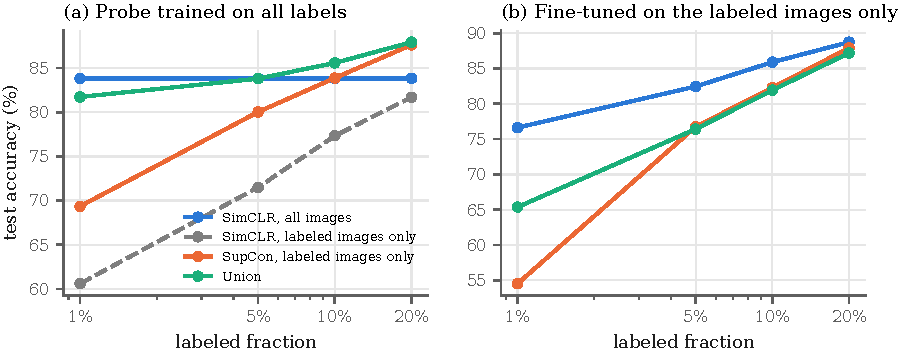
\includegraphics[width=\linewidth]{figures/fig_fraction.pdf}
\caption{Label-fraction sweep at 9,700 steps (one seed for $f\neq10\%$). Label-only methods pretrain on the
labeled images only. \textbf{(a)} With a probe trained on all labels, label-only \supcon needs a large labeled
pool. \textbf{(b)} With only the labels that exist, fine-tuning \simclr is the best use of them at every fraction.}
\label{fig:fraction}
\end{figure}

\begin{table}[t]
\centering
\small
\caption{Label-fraction sweep (seed 0, 9,700 steps). Left: probe with all labels. Right: fine-tuning with the
labeled subset only. \simclr (all images) uses no labels in pretraining, so one encoder serves every column.}
\label{tab:fraction}
\begin{adjustbox}{max width=\linewidth}
\begin{tabular}{l cccc cccc}
\toprule
 & \multicolumn{4}{c}{linear probe, all labels} & \multicolumn{4}{c}{fine-tuned, labeled subset only} \\
\cmidrule(lr){2-5}\cmidrule(lr){6-9}
labeled fraction & 1\% & 5\% & 10\% & 20\% & 1\% & 5\% & 10\% & 20\% \\
\midrule
SimCLR (all images) & 83.8 & 83.8 & 83.8 & 83.8 & 76.6 & 82.4 & 85.9 & 88.7 \\
SimCLR (labeled images only) & 60.6 & 71.5 & 77.3 & 81.7 & -- & -- & -- & -- \\
SupCon (label-only) & 69.3 & 80.0 & 83.9 & 87.6 & 54.5 & 76.7 & 82.3 & 87.9 \\
Union & 81.7 & 83.8 & 85.6 & 87.9 & 65.4 & 76.4 & 81.9 & 87.2 \\
\bottomrule
\end{tabular}

\end{adjustbox}
\end{table}

\section{Mechanism: memorised classes and missing coverage}
\label{sec:geometry}

\begin{figure}[t]
\centering
\begin{minipage}[c]{0.45\linewidth}
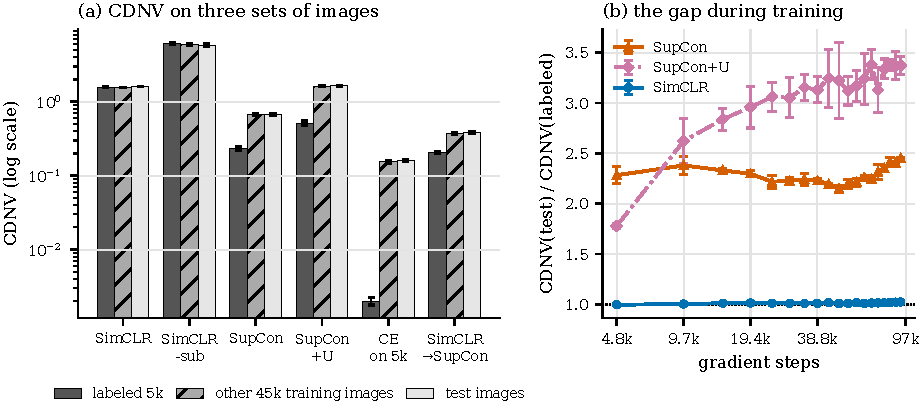
\includegraphics[width=\linewidth]{figures/fig_geometry.pdf}
\end{minipage}\hfill
\begin{minipage}[c]{0.52\linewidth}
\caption{Tightness of class clusters (CDNV; \citealp{galanti2022role}) on images that were in the
pretraining pool (solid) and on images that were not (hatched), after 9,700 steps. For label-only methods
``unseen'' are the 45,000 training images outside the pool; for full-pool methods the test set. Label-only
\supcon collapses the classes of its 5,000 images, but much of that collapse does not carry over to new
images; \simclr shows no gap.}
\label{fig:geometry}
\end{minipage}
\end{figure}

\paragraph{Collapse that does not generalise.}
The supervised contrastive loss asks every image of a class to move towards every other image of the class.
On a finite pool this can be achieved by memorising. We measure it with the class-distance normalised
variance (CDNV) of \citet{galanti2022role}, which divides the spread of a class by the squared distance
between class means, separately on images seen and unseen during pretraining (\cref{fig:geometry,tab:geometry}).
Label-only \supcon makes very tight clusters of its own images (CDNV \supconCdnvSeen, against
\simclrCdnvSeen for \simclr), but on unseen images of the same classes its CDNV is \supconCdnvHeld, a
\supconCdnvRatio-fold increase. \simclr has no such gap (ratio \simclrCdnvRatio). This is the generalisation gap
of neural collapse that \citet{hui2022limitations} found for supervised classifiers.

\paragraph{Why spent labels cannot be reused.}
The same memorisation explains \cref{sec:decompose}. A linear probe trained on the 5,000 labeled images
reaches \supconProbeTrain\% training accuracy on the \supcon encoder and \unionProbeTrain\% on the \union
encoder, against \simclrProbeTrain\% on \simclr. The CDNV of the labeled images is \supconCdnvLab (\supcon) and
\unionCdnvLab (\union), against \simclrCdnvLab (\simclr). The classes of the labeled images are already
separated, so neither the probe nor fine-tuning receives much of an error signal from them; for \simclr the
labels are new information, and fine-tuning can use them to reshape the encoder.

\paragraph{Why the plateau: coverage, not spread.}
Our report explained the weakness of label-only \supcon by ``reduced semantic diversity'' of the 10\% subset,
and the reviewer asked us to make this measurable. We embed all images with a fixed reference encoder (\simclr
on all images, seed 0) and compute several diversity statistics of each pool (\cref{tab:diversity}).
The average distance between augmented views of a class, the metric suggested by the reviewer, is
\spreadOne for a random 1\% subset, \spreadTen for 10\% and \spreadFull for the full set: a random subset is
exactly as spread out as the data it came from, because spread is a property of the distribution. What a small
pool lacks is \emph{coverage}: the distance from an unseen image to the closest pool image of its class falls
from \radiusOne (1\%) to \radiusTen (10\%) and \radiusFull (all images). Memorised clusters only help unseen
images that fall close to a memorised one, so coverage, not spread, is the property that should limit
label-only \supcon.

To separate coverage from pool size, we built three pools with exactly 500 images per class (\cref{app:pools}).
\emph{Redundant} pools are made of tight clumps of near-duplicates ($k=10$ or $50$ images per clump); the
\emph{$k$-center} pool greedily adds the image farthest from everything chosen so far \citep{sener2018coreset}.
Redundancy behaves as coverage predicts: the clumpier the pool, the worse its coverage and the worse label-only
\supcon (\clTenAcc for $k=10$ and \clFiftyAcc for $k=50$, against \supconLin for a random pool; with the probe
trained on the pool's own labels, \clTenLabAcc and \clFiftyLabAcc against \supconLabAcc). The $k$-center pool is
the informative exception. It has by far the largest spread (\spreadKc) and the worst coverage of typical test
images (radius \radiusKc, like a random pool of only \neffKc images), because it is made of atypical images.
Under the all-label probe its \supcon encoder is almost as good as the random pool's (\kcAcc); only under the
probe trained on its own labels does it drop (\kcLabAcc), because a classifier fit to atypical images transfers
poorly to typical ones.

The same pools tell a different story without labels (last column of \cref{tab:diversity}). \simclr on the
$k$-center pool collapses to \subKcAcc, far below the random pool (\subLin), exactly as its poor coverage
predicts, while redundancy does not hurt it at all (\subClFiftyAcc for $k=50$). Labels change which images are
useful: for \simclr an atypical image is just an outlier, for \supcon a labeled atypical image marks where a
class ends, and a clump of near-duplicates with the same label adds positives that are trivially easy. No single
statistic predicts both methods. Spread, the metric we were asked to compute, fails everywhere. Coverage
explains the effect of pool size, the collapse of \simclr on the $k$-center pool and the cost of redundancy for
\supcon, but not \simclr's indifference to redundancy or \supcon's tolerance of atypical labeled images: the
value of a labeled pool depends on how its labels will be used (\cref{fig:coverage,tab:diversity}).

\begin{figure}[t]
\centering
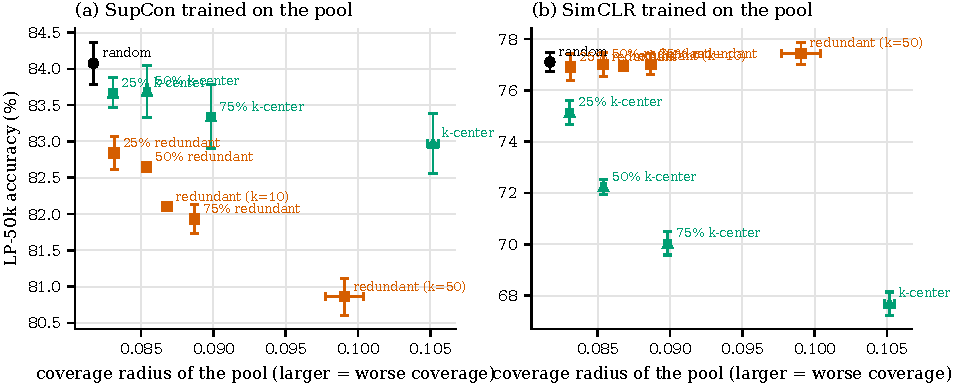
\includegraphics[width=\linewidth]{figures/fig_coverage.pdf}
\caption{Accuracy of label-only \supcon (filled) and of \simclr trained on the same pool without labels
(hollow) against two diversity measures of the pool (9,700 steps, one seed per pool, probe with all labels):
random pools of 1--20\% and three pools of exactly 5,000 images. \textbf{(a)} Coverage radius:
mean cosine distance from a test image to the nearest pool image of its class in a fixed reference feature
space (lower is better; axis reversed). \textbf{(b)} Within-class spread of augmented views.}
\label{fig:coverage}
\end{figure}

\begin{table}[t]
\centering
\small
\caption{Diversity of labeled pools in the reference feature space (seed 0) and the linear-probe accuracy of
label-only \supcon trained on each pool for 9,700 steps.}
\label{tab:diversity}
\begin{adjustbox}{max width=\linewidth}
\begin{tabular}{l r cccc cc c}
\toprule
 & & \multicolumn{4}{c}{diversity of the pool} & \multicolumn{2}{c}{SupCon on the pool} & SimCLR on the pool \\
\cmidrule(lr){3-6}\cmidrule(lr){7-8}\cmidrule(lr){9-9}
pool & images & spread (pairs) & spread (aug.\ views) & Vendi & coverage radius & probe, 50k & probe, own labels & probe, 50k \\
\midrule
random 1\% & 500 & 0.358 & 0.391 & 5.0 & 0.1242 & 69.3 & 56.2 & 60.6 \\
random 5\% & 2,500 & 0.356 & 0.387 & 5.8 & 0.0912 & 80.0 & 75.7 & 71.5 \\
random 10\% & 5,000 & 0.353 & 0.385 & 5.9 & 0.0817 & 83.9 & 81.2 & 77.3 \\
random 20\% & 10,000 & 0.352 & 0.384 & 6.0 & 0.0729 & 87.6 & 86.5 & 81.7 \\
random 100\% & 50,000 & 0.351 & 0.383 & 6.0 & 0.0569 & -- & -- & 83.8 \\
redundant ($k{=}10$) & 5,000 & 0.335 & 0.369 & 5.1 & 0.0868 & 82.1 & 78.3 & -- \\
redundant ($k{=}50$) & 5,000 & 0.315 & 0.351 & 4.5 & 0.1006 & 80.6 & 72.9 & 77.2 \\
$k$-center & 5,000 & 0.426 & 0.453 & 9.5 & 0.1048 & 83.4 & 77.0 & 67.6 \\
\bottomrule
\end{tabular}

\end{adjustbox}
\end{table}

\begin{table}[t]
\centering
\small
\caption{Geometry of the encoder features after 9,700 steps (mean over seeds). CDNV on seen and unseen images;
on the test set, accuracy of the nearest-class-centre rule with centres from the seen images, mean deviation of
the angles between centred class means from those of a simplex ETF, and coefficient of variation of their norms.}
\label{tab:geometry}
\begin{tabular}{l ccc ccc}
\toprule
 & \multicolumn{3}{c}{CDNV $\downarrow$} & \multicolumn{3}{c}{test set} \\
\cmidrule(lr){2-4}\cmidrule(lr){5-7}
method & seen & unseen & ratio & NCC acc. & ETF dev.\ $\downarrow$ & equinorm CV $\downarrow$ \\
\midrule
SimCLR & 1.21 & 1.23 & 1.0$\times$ & 74.2 & 0.226 & 0.224 \\
SimCLR (subset) & 2.37 & 2.43 & 1.0$\times$ & 59.7 & 0.160 & 0.311 \\
SupCon (label-only) & 0.17 & 0.52 & 3.1$\times$ & 80.4 & 0.100 & 0.252 \\
Union & 1.54 & 1.60 & 1.0$\times$ & 77.9 & 0.196 & 0.236 \\
\bottomrule
\end{tabular}

\end{table}

\finding{Label-only \supcon memorises its labeled pool: its classes are \supconCdnvRatio times tighter on seen than
on unseen images, and the labels it memorised are of little further use downstream. A random labeled subset is as
spread out as the full data; what it lacks is coverage of unseen images.}

\section{Comparison with established methods}
\label{sec:baselines}

\begin{table}[t]
\centering
\small
\caption{Baselines on the same CIFAR-10 split with 10\% labels (ResNet-18, 9,700 steps or the same number of
processed images, one seed unless an s.d.\ is shown). $^\ddagger$Accuracy with only the 5,000 labels:
fine-tuning for the pretrained encoders, the trained classifier (EMA weights) for CE, MixMatch and FixMatch.
$^\S$MixMatch and FixMatch are trained for about 1\% of the steps of the original papers, which report 93.8\%
and 95.7\% with 4,000 labels and a Wide ResNet-28-2 \citep{sohn2020fixmatch}.}
\label{tab:baselines}
\begin{adjustbox}{max width=\linewidth}
\begin{tabular}{l l c ccc}
\toprule
method & family & labels used & linear (all labels) & $k$NN & accuracy with 5k labels$^\ddagger$ \\
\midrule
Supervised CE & supervised & 5k & 82.9 & 82.5 & 82.4 \\
SimCLR & contrastive SSL & -- & 83.8{\scriptsize$\pm$0.1} & 79.9{\scriptsize$\pm$0.1} & 85.9{\scriptsize$\pm$0.4} \\
BYOL & non-contrastive SSL & -- & 86.1 & 82.9 & 85.8 \\
SimSiam & non-contrastive SSL & -- & 76.9 & 71.1 & 82.5 \\
SupCon (label-only) & supervised contrastive & 5k & 83.9{\scriptsize$\pm$0.1} & 82.0{\scriptsize$\pm$0.1} & 82.3{\scriptsize$\pm$0.1} \\
MixMatch$^\S$ & semi-supervised & 5k & 92.6 & 92.7 & 92.4 \\
FixMatch$^\S$ & semi-supervised & 5k & 91.4 & 90.8 & 90.8 \\
Union & semi-supervised contrastive & 5k & 85.6{\scriptsize$\pm$0.2} & 83.3{\scriptsize$\pm$0.4} & 81.9{\scriptsize$\pm$0.4} \\
Supervised CE, all labels (reference) & supervised & 50k & 94.7 & 94.8 & 94.8 \\
\bottomrule
\end{tabular}

\end{adjustbox}
\end{table}

\Cref{tab:baselines} places the encoders among other families, all trained with the same 5,000 labels and the
same image budget. Three points are worth stating plainly.

\emph{\simclr is a reasonable self-supervised baseline at this budget}: BYOL reaches \byolLin and SimSiam
\simsiamLin, against \simclrLin. With 1,000 epochs, published ResNet-18 numbers on CIFAR-10 are 90--94\%
\citep{dacosta2022sololearn}, so all our contrastive numbers are those of a short schedule.

\emph{If the goal is the best classifier from 5,000 labels, use a semi-supervised method.} Given the same
number of processed images as a 9,700-step contrastive run, MixMatch reaches \mixmatchAcc and FixMatch
\fixmatchAcc, above every contrastive pipeline in this paper, including \simclr fine-tuned after twice as many
steps (\simclrTwoHundredFt). Both remain below their published accuracy, which they reach after about a
million steps.

\emph{Labels in the loss make pretraining no better than plain supervision.} A network trained with
cross-entropy on the 5,000 labeled images alone, for the same 9,700 steps, reaches \ceTen. This is as good as
label-only \supcon followed by fine-tuning (\supconFt) and \union followed by fine-tuning (\unionFt): once the
labels are inside the contrastive loss, neither the contrastive objective nor the 45,000 unlabeled images add
measurable accuracy for a user who has only those labels. What clearly improves on plain supervision is
pretraining \emph{without} labels and fine-tuning afterwards: \simclrFt with \simclr and \byolFt with BYOL.

\emph{These baselines fit our explanation.} MixMatch and FixMatch also use the labels from the first step, but
they do not ask the network to cluster the labeled images; they turn the network's predictions into targets for
the unlabeled images (sharpened guesses or confident pseudo-labels), so the supervision keeps flowing to images
that have not been memorised. Label-only \supcon and
\union spend the labels on the 5,000 labeled images themselves. Our claims are therefore about how to use labels
\emph{inside contrastive pretraining}, the setting in which one encoder is pretrained once and reused; they are
not claims about the best achievable accuracy with 5,000 labels.

\paragraph{Other datasets and architectures.}
\Cref{tab:generalization} repeats the four configurations on CIFAR-100 and with a ResNet-50 on CIFAR-10 (one
seed each, 9,700 steps). CIFAR-100 is the harder case for label-only pretraining: 10\% of the labels means only
50 labeled images per class. Already at 9,700 steps \simclr is ahead under the all-label probe (\cHundredSimclr
vs.\ \cHundredSupcon), and with only the labels that exist the gap is large: fine-tuned \simclr reaches
\cHundredSimclrFt, against \cHundredSupconFt for \supcon and \cHundredUnionFt for \union. A ResNet-50 trains more slowly,
so 9,700 steps is still in the regime where labels in the loss help the all-label probe (\rFiftySupcon for
\supcon and \rFiftyUnion for \union, against \rFiftySimclr for \simclr). With only the labels that exist, the
ordering is the same as for the ResNet-18: fine-tuned \simclr reaches \rFiftySimclrFt, against \rFiftySupconFt for
\supcon and \rFiftyUnionFt for \union.

\begin{table}[t]
\centering
\small
\caption{The four configurations on CIFAR-100 (ResNet-18) and with a ResNet-50 on CIFAR-10 (one seed,
10\% labels, 9,700 steps). ``Probe, 50k'' and $k$NN use all training labels; ``fine-tune, 5k'' and ``probe, 5k''
use only the labeled 10\%.}
\label{tab:generalization}
\begin{tabular}{l ccc ccc}
\toprule
 & \multicolumn{3}{c}{CIFAR-100, ResNet-18} & \multicolumn{3}{c}{CIFAR-10, ResNet-50} \\
\cmidrule(lr){2-4}\cmidrule(lr){5-7}
method & probe, 50k & $k$NN & fine-tune, 5k & probe, 50k & $k$NN & fine-tune, 5k \\
\midrule
SimCLR & 54.2 & 42.6 & 51.8 & 85.8 & 80.4 & 85.6 \\
SimCLR (subset) & 44.6 & 37.1 & -- & -- & -- & -- \\
SupCon (label-only) & 50.5 & 48.9 & 44.7 & 86.4 & 84.1 & 83.6 \\
Union & 56.1 & 51.7 & 46.8 & 87.2 & 84.2 & 82.4 \\
\bottomrule
\end{tabular}

\end{table}
